\SECTION{Evaluation}\label{sec:evaluation}
Here, we evaluate scheduling overhead and scheduling performance.
Scheduling experiments are limited to GPU scheduling because CPU scheduling performance has already been examined experimentallys~\cite{kato2009loadable}.
In this evaluation, we focus on two points,
identifying Linux-RTXG’s disadvantages and demonstrating the quality of service (QoS) performance.
\if 0
Real-world oriented applications using GPUs~\cite{hirabayashi:cpsna2013,tokamak} were executed periodically.
These evaluation applications are equivalent to the real-world oriented applications
because GPU applications characteristics are these application on the single GPU kernel.
\fi
We compare the functions and features of the proposed method and previous methods in a qualitative evaluation in the next section.
\SUBSECTION{Experimental Environment}
Our experiments were conducted using Linux kernel 3.16.0, an NVIDIA Geforce GTX680 GPU, a 3.40 GHz Intel Core i7 2600 (8 cores, including two hyperthreadling cores), and 8 GB main memory.
GPU programs were written in CUDA and compiled by NVCC v6.0.1.
We used the NVIDIA 331.62 driver and Nouveau Linux-3.16.0 driver.
In addition, we used NVIDIA CUDA-6.0 libraries and Gdev.

\SUBSECTION{Interrupt intercept overhead}
We measured the interrupt interception overhead using the Nouveau GPU driver to compare and identify the type of interrupt.
We compared elapsed time from the beginning to the end of the ISR.

\begin{figure}[t]
\begin{center}
\includegraphics[width=0.4\textwidth]{img/interrupt}
\caption{Interrupt intercept overhead}
\label{fig:irq_overhead}
\end{center}
\end{figure}
\begin{figure}[t]
\begin{center}
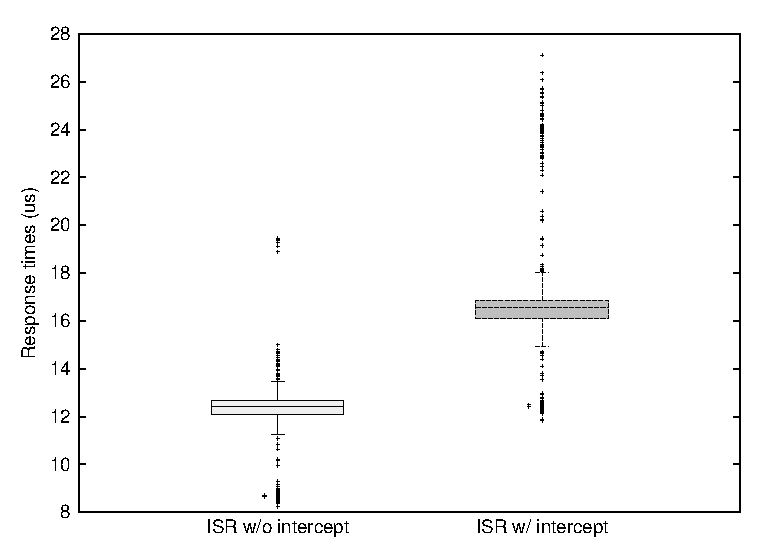
\includegraphics[width=0.4\textwidth]{img/interrupt_response}
\caption{Comparison of the response time of interrupt processing with and without intercept}
\label{fig:response}
\end{center}
\end{figure}
\begin{figure}[t]
\begin{center}
\includegraphics[width=0.4\textwidth]{img/tasklet_vs_interrupt}
\caption{Comparison of the response time of the top-half and bottom-half of the interrupt handler}
\label{fig:bottomvstasklet}
\end{center}
\end{figure}

Figure~\ref{fig:irq_overhead} shows the results of measurements for the above setting.
Here, Raw ISR is the ISR executed in the original routine.
Note that ISR Intercept is the only intercept considered in our approach.
ISR Intercept w/Func refers to interception with processing functions that identify the ISR and wake the scheduler thread.
The results shown are average times (1000 executions); error bars indicate minimum and maximum values.

From the results, it is evident that overhead exists.
Overhead for ISR Intercept was 247 ns, which is 0.8\% of the total time required for the Raw ISR process.
Overhead for ISR Intercept w/Func was 790 ns, which is 2.6\% of the total time required for the Raw ISR process.
Intuitively, these overheads unlikely to affect the system because are very small values;
however, interrupts (e.g., timer interrupts) occur frequently, and cumulatively are likely to be significant.

Next, we compare response times to determine the impact of the interrupt intercept.
The response times are elapsed times from the start of interrupt processing to the end of identify the each interrupt type (e.g., timer, compute, FIFO, and GPIO).
The response times for ISRs with and without intercepts are shown in Figure~\ref{fig:response}.
Response times with intercepts were approximately 1.4 times longer than response times for interrupts without intercepts.
However, we target systems that do not use the GPU runtime resource management features.
Therefore, we should aim to fast response time of intercepted ISR, and original ISR response time is slow there is not affected much.

We also evaluated response time of the ISR (top-half) and the tasklet (bottom-half) in an environment to compare our results with those of previous approaches.
GPUSync intercepts the $tasklet\_schedule()$ if it is called by the NVIDIA driver.
We compare the response times of a tasklet intercept using GPUSync and the ISR intercept.
This evaluation measured response time until the responsible timing from the start of interrupt process which is $do\_IRQ$ function is called.
Figure~\ref{fig:bottomvstasklet} shows the result of this evaluation.
As can be seen, the tasklet interception response time is worse than the ISR time.
This occurs because the tasklet is typically called after significant ISR processing.

\SUBSECTION{Independent Synchronization Mechanism Overhead}
We evaluated the overhead relative to the use of an independent synchronization mechanism.
Such a mechanism must call $rtx\_nvrm\_notify()$ at the time of requested synchronization (e.g., after the kernel launch request) and $rtx\_nvrm\_init()$.
In vanilla environments, Linux-RTX’s APIs are not necessary.
Therefore, overhead includes the API execution time.
We measured overhead by measuring API execution time between each API call and return.

\begin{figure}[!t]
\begin{center}
\subfigure[Part of Initialize]{\includegraphics[width=0.23\textwidth]{img/irq_rise_init.eps}}\subfigure[Part of notify]{\includegraphics[width=0.22\textwidth]{img/irq_rise_notify.eps}}
\caption{Interrupt raised method overhead}
\label{fig:irq_rise_overhead}
\end{center}
\end{figure}

Figure~\ref{fig:irq_rise_overhead} shows the measurement results.
Initilize part is required to call a Linux process to allocate an indirect buffer and registers several engines such as compute and copy to the device driver.
Notify part (NOTIFY and FENCE) insert commands into a command steram to GPU devices that are called when synchronization is required, such as after a kernel launch is issued.
Execution time have scatters that are affected by an ioctl system call.
%結果をFigure \ref{fig:irq_rise_overhead}に示す。
%InitializeはIndirect Bufferはプロセスが立ち上がるたびに、
%コマンド送信用のIndirect Bufferの確保や各エンジンの登録のために呼び出される必要がある。
%Notifyはカーネル実行後や非同期メモリコピー実行後のような同期を発生させたいタイミングで呼び出される。
%これらはioctlシステムコールによってユーザ空間とカーネル空間をまたいでる影響か、実行時間のバラ付きが大きく出ている。
The average Initizalize time is approximately 4 ms.
However, applications are not affected significantly because Initialize is only called once.
Notify’s NOTIFY requires approximately 3.5 μs and FENCE requires approximately 2 μs.
Consequently, the time required by these method is not a major consideration for applications.
However, overhead must be considered in a shot application cycle.

\SUBSECTION{Scheduling Overhead}\label{sec:eval:sched_overhead}

\if 0
\begin{figure}[t]
\begin{center}
\includegraphics[width=1.5\textwidth]{img/sum_task_fp.eps}
\caption{Scheduling overhead(between GPU kernel launch request and synchronization)}
\label{fig:fp_overhead}
\end{center}
\end{figure}
\fi

\begin{figure}[t]
\begin{center}
\includegraphics[width=.44\textwidth]{img/sum_task.eps}
\caption{Scheduling overhead (Time of entire task)}
\label{fig:fp_task_overhead}
\end{center}
\end{figure}

We evaluated scheduling overhead using the proposed Linux-RTXG scheduler.
We prepared three applications, i.e., vanilla, mutex, and rtx to measure overhead.
These applications are based on a common application that is Gdev’s microbenchmark, which has a GPU looping function.
%details
Changes were arranged to generate multiple GPU tasks by the $fork()$ systemcall.
Each task has 10 jobs, and each job includs GPU data transfer and GPU kernel execution.
The rtx application was scheduled by rtx.
The mutex application was limited to a single kernel issue by exclusion control using mutex similar to rtx.
The vanilla application was not changed.
The CPU scheduling policy used in this evaluation was the simple fixed-priority scheduling of the proposed Linux-RTXG, which is similar to Linux’s $SCHED\_FIFO$. Note that the difference between these policies is the presence or absence of job management.
The GPU scheduling policy is fixed-priority scheduling with resrouce reservation, i.e., BAND scheduling policy.
Here, synchronization is used NOTIFY of the independent synchronization mechanism.

We measured the average time in 100 times GPU task execution (1000 jobs).
The result show in Figure~\ref{fig:fp_task_overhead}.
\if 0
The launch\_advice is time of until GPU kernel launch request is accept on the Linux-RTXG.
The mutex is time to get the mutex lock.
The sync is time of untile synchronizationed from issued the GPU kernel launch issue.
\fi

Overhead increases in proportion as the number of tasks increases because task scheduling processing times is increased.
Max overhead is 10\% at the eight tasks based on "vanilla" time.

%%
%The most factors contained in the overhead is the API's overheads and scheduling algorithms (e.g. Band scheduling include yield times).
%If application periods is short, users are conscious of the overheads.

%launch\_adviceはrtx\_gpu\_launchによってGPU利用のためのリクエストを出してから、許可がでるまでを示しており、
%get\_mutexはmutexによってロックを獲得するまでの時間、
%launch、notifyはそれぞれコマンドを発行するまでにかかった時間で、
%syncは発行されてから同期完了するまでの時間である。
%全て、100回のアプリケーション実行($number of tasks ☓$)の平均値である.

%rtxでスケジューリングした場合のオーバヘッドを測定するために、"vanilla", "mutex", "rtx"の3種類のアプリケーションを用意した。
%全てに共通するのが、1個のアプリケーションに複数のタスクが存在しており、
%各タスクには10個のジョブが含まれることである。1個のジョブはGPUへのデータ転送、GPUカーネル実行、GPUからのデータ転送を含んでいる。GPUカーネルは単純な行列の計算を行う。
%
%3種で異なる点として、まずmutexは同時にlaunchが発行されるのが1つに調停されるようにmutexを用いてロックしたバージョンである。
%そしてrtxはlinxu-rtxgを用いて実行したケースであり、
%vanillaはそれらの追加が無くスケジューリングや調停を一切行わないケースである。


%CPUのスケジューリングはlinux-rtxを用いたシンプルなFixed-priorityスケジューリング (LinuxのSCHED\_FIFOと同様のポリシー、ジョブ管理のみを行う)を用いる。
%GPU側のスケジューリングは、Gdevで提案されたBANDスケジューラ、Linux-RTXでの同期は全てNOTIFYを用いて行う。


\SUBSECTION{Performance of QoS management}
Experiments were also performed to evaluate QoS management performance.
In this evaluation, we measured the utilization of each tasks in several environments,
which indicates whether performance is affected by kernel modification.
\begin{figure}[!t]
\begin{center}
\subfigure[FIFO Scheduling]{\includegraphics[width=0.4\textwidth]{img/fifo_rtx_nvidia}} 
\label{fig:fifo_rtx_nvidia} \\
\subfigure[BAND Scheduling]{\includegraphics[width=0.4\textwidth]{img/band_rtx_nvidia}}
\label{fig:band_rtx_nvidia}
\caption{Utilization of two tasks with the Linux RTXG scheduler (NVIDIA driver). Each task had different workloads and different resources allocations(VGPU0 = 40\%, VGPU1 = 60\%).}
\label{fig:rtx_nvidia}
\end{center}
\end{figure}

\begin{figure}[!t]
\begin{center}
\subfigure[FIFO Scheduling]{\includegraphics[width=0.4\textwidth]{img/fifo_rtx}}
\label{fig:fifo_rtx} \\
\subfigure[BAND Scheduling]{\includegraphics[width=0.4\textwidth]{img/band_rtx}}
\label{fig:band_rtx}
\caption{Utilization of two tasks with the Linux RTXG scheduler (Nouveau driver). Each task had different workloads and different resource allocations (VGPU0 = 40\%, VGPU1 = 60\%).}
\label{fig:rtx_nouveau}
\end{center}
\end{figure}

\begin{figure}[t]
\begin{center}
\includegraphics[width=0.5\textwidth]{img/band_rtx_fair}
\caption{Utilization of four tasks with the Linux-RTXG's BAND VGPU scheduling. Each tasks had a equal workload and a equal GPU resource allocation.}
\label{fig:band_rtx_fair}
\end{center}
\end{figure}

\if 0
\begin{figure}[t]
\begin{center}
\includegraphics[width=0.5\textwidth]{img/band_rtx_diff}
\caption{Utilization of four tasks with the Linux-RTXG's BAND VGPU scheduling. Each tasks had a different workload and a different resources.}
\end{center}
\label{fig:band_rtx}
\end{figure}
\fi

\if 0
\begin{figure}[t]
\begin{center}
\includegraphics[width=0.5\textwidth]{img/dummy}
\caption{Utilization of four tasks with the G. All tasks are fairy given resources which is 25\%}
\end{center}
\label{fig:qos_gdev}
\end{figure}
\fi

QoS performance use an indication of whether the task of the resource is guaranteed.
We evaluate task isolation performances with Linux-RTXG’s GPU scheduler using the NVIDIA GPU driver and the Nouveau GPU driver to confirm the guaranteed resources.
First, we measured the utilization when running two GPU tasks.
Each GPU tasks had a different workload and a different GPU resource.
One GPU task was allocated VGPU0, and given the 40\% GPU resource.
This task has about 1.2 times the workload of other tasks.
The other GPU task was allocated VGPU1 and given the 60\% GPU resource.
VGPU1 task was scheduled to start approximately 5 safter the VGPU0 task.

The NVIDIA GPU driver results are shown in Figures~\ref{fig:rtx_nvidia}.
The FIFO scheduling policies are shown in Figure~\ref{fig:rtx_nvidia}(a),
and the BAND scheduling policies are shown in Figure~\ref{fig:rtx_nvidia}(b).
The Nouveau GPU driver results are shown in Figures~\ref{fig:rtx_nouveau}.
The FIFO scheduling policies shown in Figure~\ref{fig:rtx_nouveau}(a),
and the BAND scheduling policies shown in Figure~\ref{fig:rtx_nouveau}(b).
The results shown in Figure~\ref{fig:rtx_nvidia}(a),~\ref{fig:rtx_nouveau}(a) indicate that the GPU tasks are performed in accordance with the workload by fair scheduling.
The results shown in Figure~\ref{fig:rtx_nvidia}(b),~\ref{fig:rtx_nouveau}(b) indicate that the GPU tasks are performed in accordance with the utilization by resource reservation mechanisms.
The VGPU1 taks’s maximum error was approximately 3\% for the initial BAND scheduling policies’ resource management using the NVIDIA GPU driver.
The VGPU0 task’s maximum error was approximately 5\%.
The VGPU1 task’s maximum error was approximately 2\% under the initial BAND scheduling policies' resource management using the Nouveau GPU driver.
The VGPU0 task’s maximum error was approximately 2\%.
Large spikes occurred due to GPU kernel overrun.
If the GPU scheduler need to large spike is reduced, the GPU scheduler is needed for runtime approaches such as making preemptive GPU kernel.

We then measured utilization running four GPU tasks.
Each GPU tasks had equal workload and equal GPU resource allocation.
In addition, each GPU task was allocated to each VGPU.
Results for BAND scheduling policies are shown in Figure~\ref{fig:band_rtx_fair}.
A maximum error of these VGPUs was appropriately 9\%, it values are occurred because of the timing of budget replenishment and a synchronization latency.  

Therefore, the results show that the synchronization mechanism of the proposed Linux-RTXG can schedule tasks without sacrificing performance.
